\section{Введение}\label{s1}
Теория интегрируемых бильярдов развивается в двух в каком-то смысле встречных направлениях:

(1) доказательство гипотезы Биркгофа; 

(2) поиск интегрируемых модификаций эллиптического бильярда.

В решении задачи (1), начиная с работы С.~В.~Болотина \cite{Bol90}, за последние годы был достигнут значительный прогресс --- упомянем здесь работы Миронова, Бялого и Драговича \cite{bm2022, bm2024}.

В направлении задачи (2) заметный прогресс связан с группой исследователей, возглавляемых А.~Т.~Фоменко (В.~В.~Ведюшкина (Фокичева) \cite{Fok15, 1},  В.~А.~Кибкало).
Объем полученных результатов здесь настолько значителен, что коротко изложить их не представляется возможным. Мы рекомендуем читателю обратиться к обзору А.~Т.~Фоменко и В.~В.~Ведюшкиной \cite{fv2023}.
Хорошо известно, что бильярд в эллипсе в присутствии постоянного магнитного поля, перпендикулярного плоскости стола, не интегрируем (физическая точка зрения отражена в большом количестве статей, в частности, см. Берри и Робник \cite{berry1985, berry1986}). 
Математически строгие утверждения, в том числе для бильярдных столов на поверхностях постоянной кривизны,  содержатся в работах \cite{bm2019, zbMATH06661562, bm2020}.
Однако, бильярд в магнитном поле в круге интегрируем и демонстрирует интересное поведение с точки зрения инвариантов интегрируемых гамильтоновых систем.

В направлении (2) отметим интересную систему, введенную Драговичем и Раднович в \cite{DraGasRad22} (так называемая <<бильярдная игра>>),  а также недавнюю работу \cite{wire}.
Кроме того, имеется цикл работ про интегрируемые бильярды с потенциалом, см. например \cite{Dra1, Dra4}, инициированный работой В.~В.~Козлова \cite{Kozlov}.

\medskip
%\subsection{}\label{s1.1}
%\begin{remark}
%Этот случай можно рассматривать как классический бильярд на невыпуклом софокусном столе по алгоритму, изложенному в \cite{moskvin}. 
%То же справедливо для бильярда с <<преломлением>>, но с оговорками.
%\textcolor{red}{Этим я хотел сказать, что теоретически можно придумать алгоритм, как у Москвина.}
%\end{remark}

Недавно авторами был обнаружен новый класс интегрируемых систем, связанный с бильярдами в областях, ограниченных софокусными квадриками.
Опишем простейшие случаи систем из этого класса.
Пусть задана область $\Omega$, ограниченная эллипсом 
$\dfrac{x^2}{a^2} + \dfrac{y^2}{b^2} = 1$, где $a > b > 0$.
Дуга софокусной квадрики $Q_{\lambda_1} = \left\{ \dfrac{x^2}{a^2-\lambda_1} + \dfrac{y^2}{b^2-\lambda_1} = 1 \right\}$ разделяет  $\Omega$ на области $\Omega_1$ и $\Omega_2$.
В случае $0 < \lambda_1 < b^2$ квадрика $Q_{\lambda_1}$ является эллипсом, а при $b^2 < \lambda_1 < a^2$ -- гиперболой.

Припишем каждой области $\Omega_i$  коэффициент $n_i,\  i=1,2$, имеющий смысл показателя преломления. 
Рассмотрим движение материальной точки в области $\Omega$. Будем считать, что на внешней границе области $\Omega$ движение подчиняется закону <<угол падения равен углу отражения>>, 
а на общей границе областей $\Omega_1$ и $\Omega_2$ выполняется модифицированный закон преломления, который мы опишем ниже в общем виде.

Пусть две области $\Omega_i$ и $\Omega_j$ граничат по кривой $C$. 
Показатели преломления для этих областей равны $n_i$ и $n_j$, соответственно.
Будем считать, что движение материальной точки при достижении кривой $C$ подчиняется следующим правилам (далее мы будем ссылаться на них как на модифицированный закон преломления $(\ast)$).
\begin{itemize}
\item[1.] Выполнено соотношение $n_i \cos \theta_i = n_j \cos \theta_j $, где $\theta_i, \theta_j \in [0,\frac{\pi}{2} ]$ -- углы, которые образуют отрезки траектории   в соответствующих областях с нормалью к кривой $C$, если $\theta_i$ и $\theta_j$ корректно определены.
\item[2.] Если $n_i > n_j$ и материальная точка, двигаясь в области $\Omega_i$, достигает кривой $C$, причем в точке пересечения траектории с кривой $C$ выполнено неравенство $\cos \theta_i > \frac{n_j}{n_i}$, то происходит полное внутреннее отражение траектории в область $\Omega_i$ по закону <<угол падения равен углу отражения>> (в этом случае угол $\theta_j$ не определен, поскольку $\frac{n_i}{n_j} \cos \theta_i > 1$). 
\item[3.] В предыдущих двух пунктах два соседних отрезка траектории с общей точкой на кривой $C$ лежат по разные стороны от нормали к кривой $C$ в этой точке.
\item[4.] Если $n_i > n_j$ и материальная точка, двигаясь в области $\Omega_j$, достигает кривой $C$, причем $\theta_j = 0$, тогда $\cos \theta_i = \frac{n_j}{n_i}$ и материальная точка продолжает движение в области $\Omega_i$ вдоль любого из двух возможных направлений, образующих угол $\theta_i$ с нормалью к кривой $C$.
\item[5.] Аналогично при $n_i < n_j$.
\end{itemize}
Для удобства будем считать, что при преломлении модуль вектора скорости не меняется.

\begin{figure}[!htb]
\minipage{0.32\textwidth}
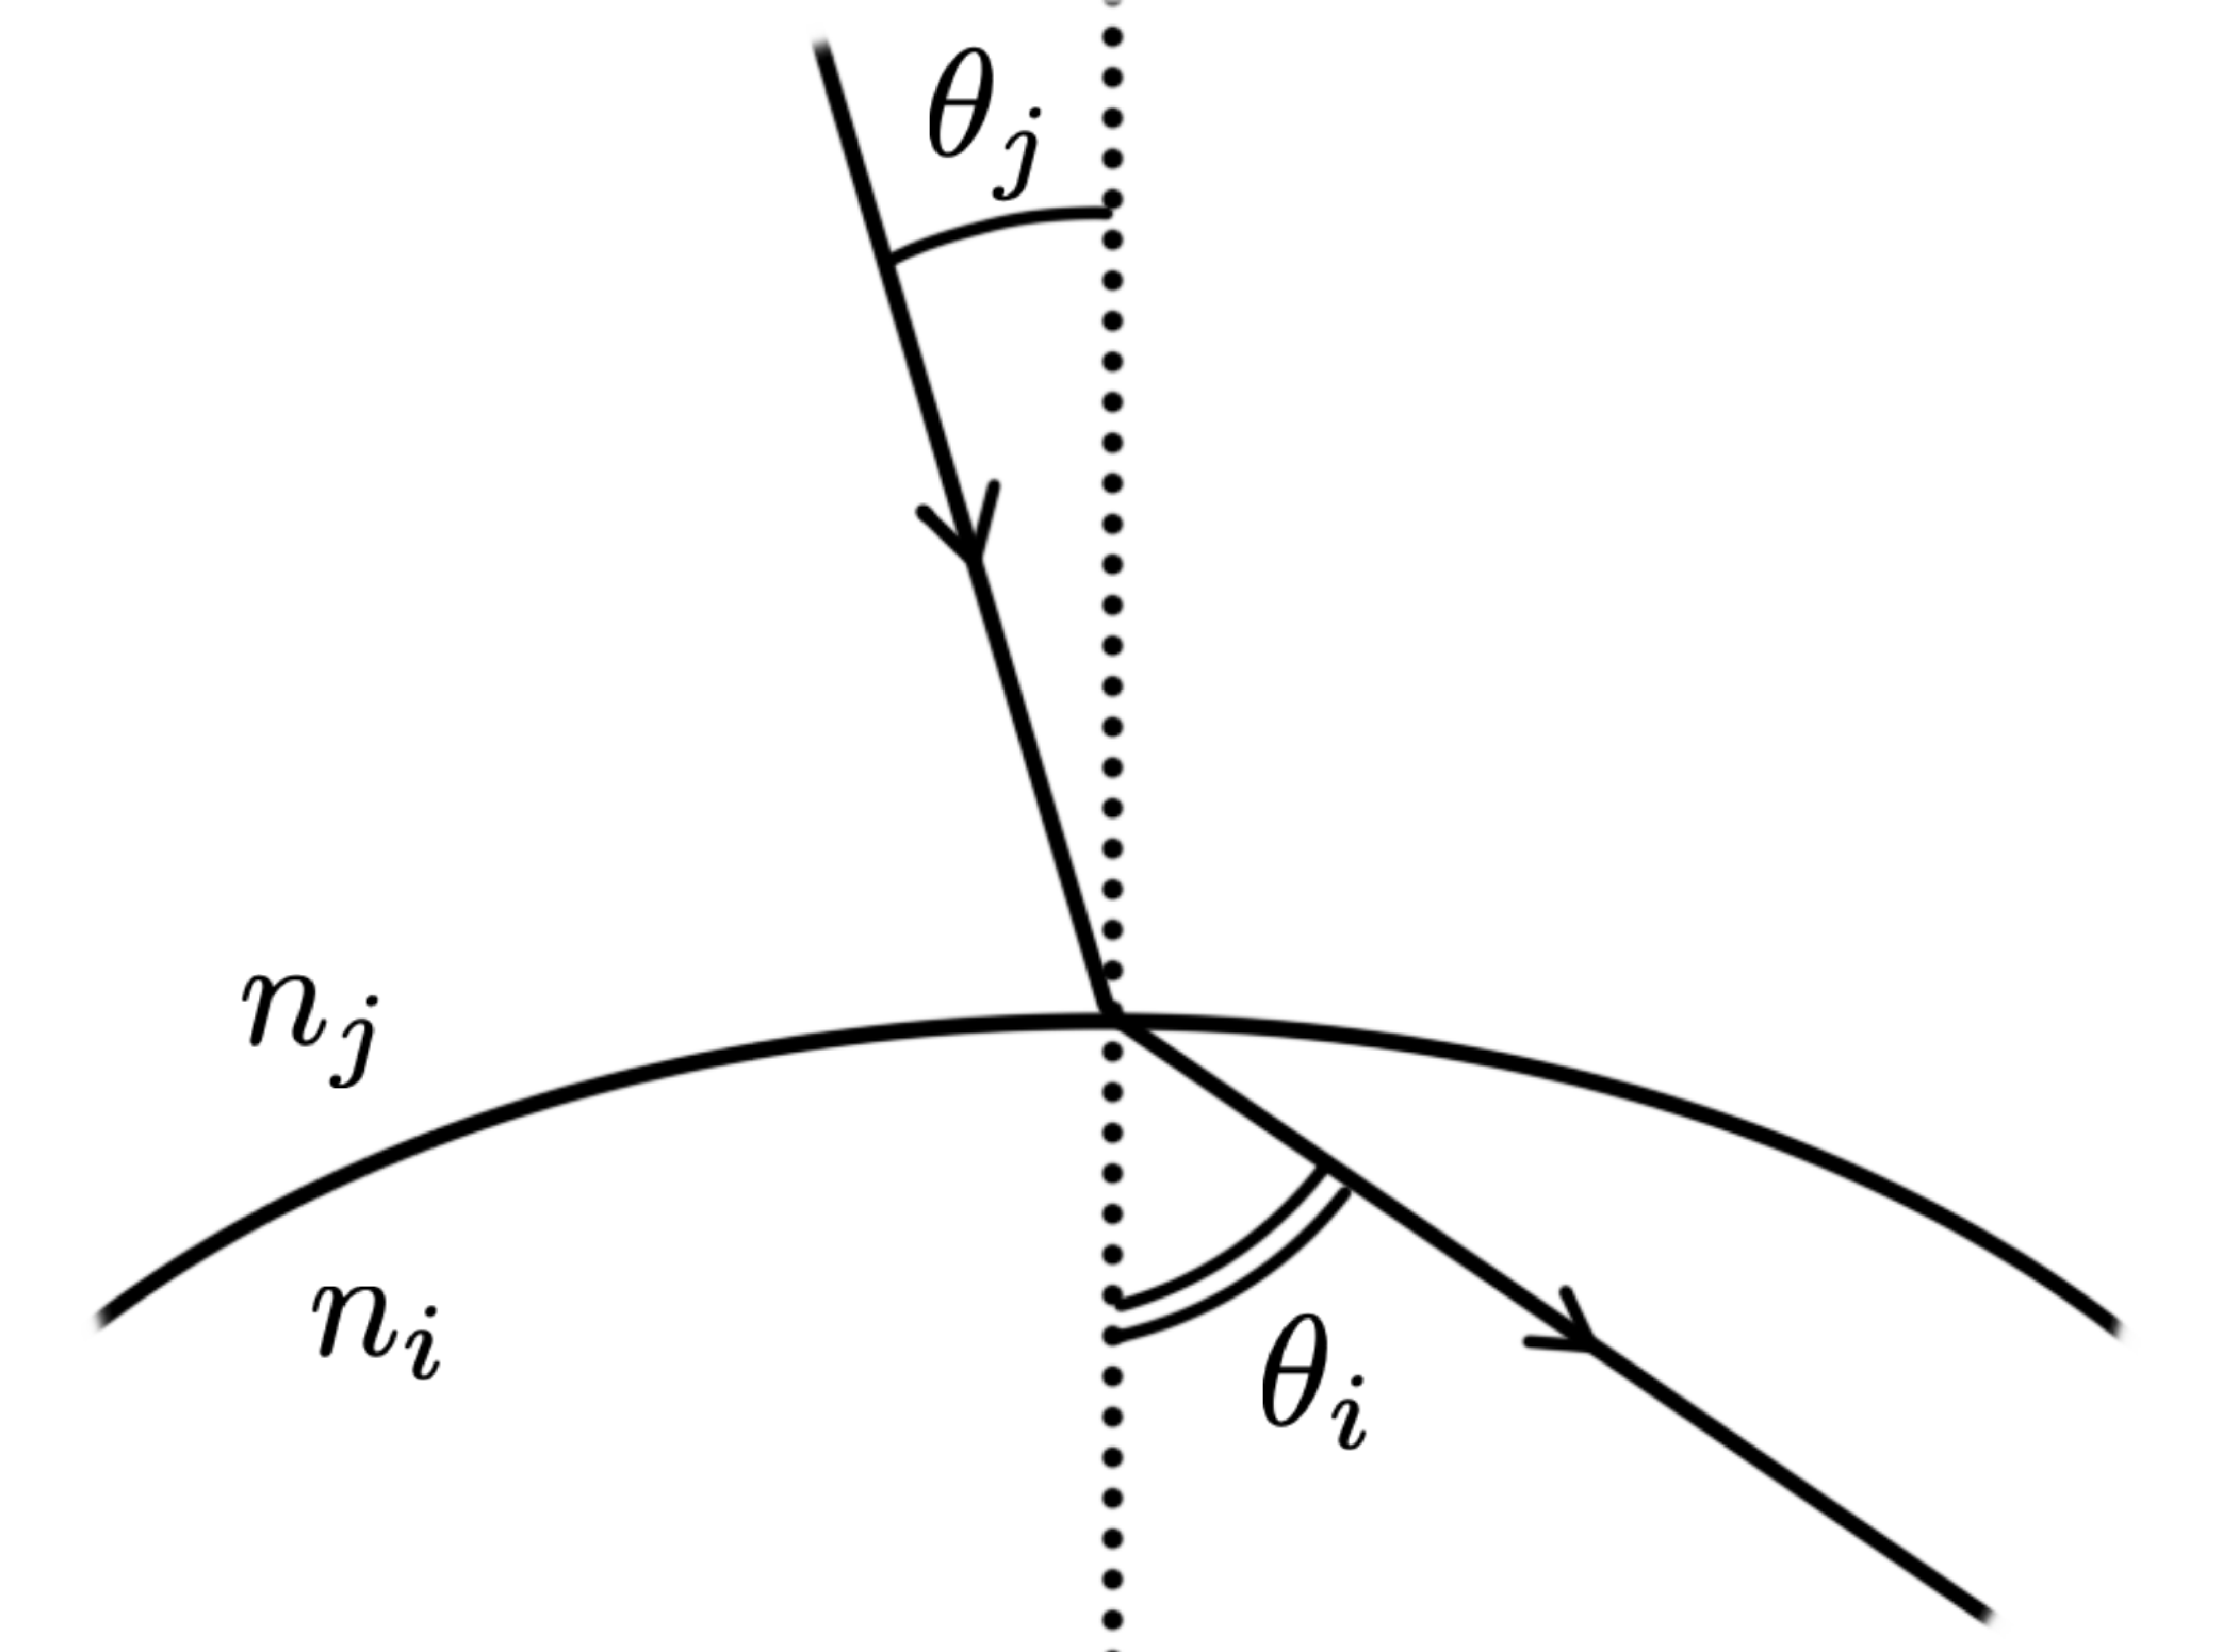
\includegraphics[width=\linewidth]{images/section1/example1.pdf}
    \caption{Иллюстрация к пункту 1.}
    \label{fig:pt8:_example1}
\endminipage\hfill
\minipage{0.32\textwidth}
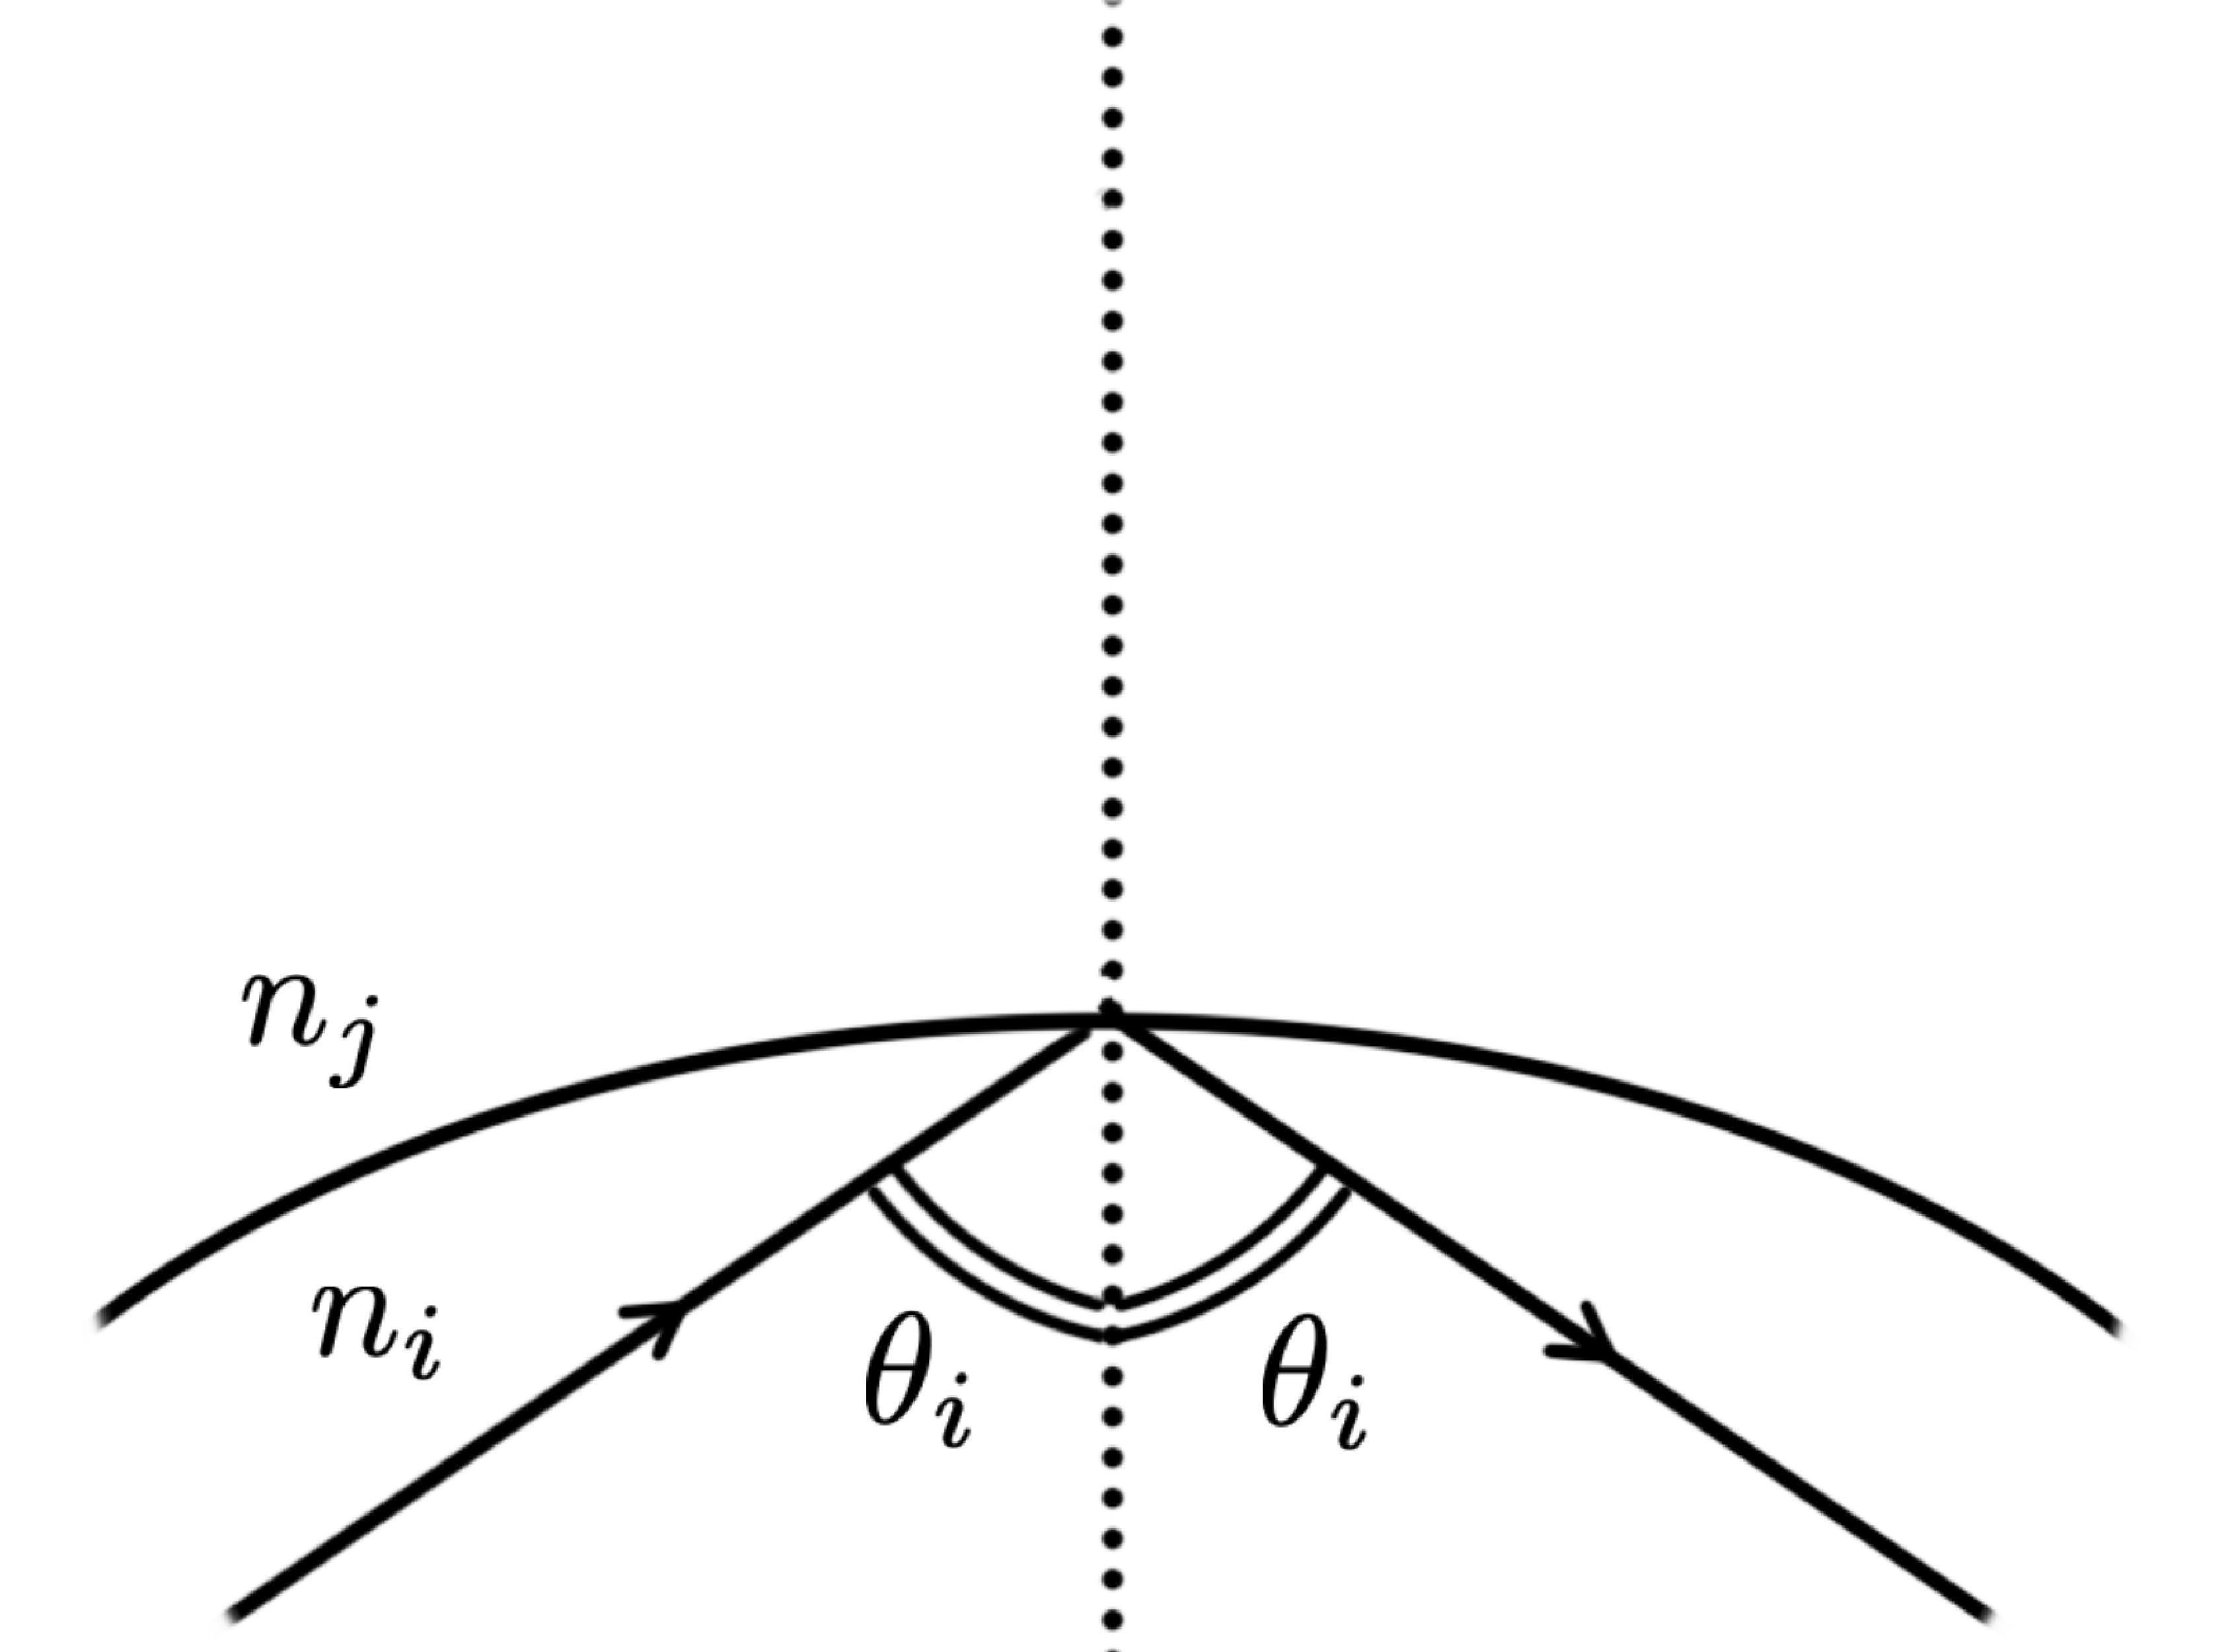
\includegraphics[width=\linewidth]{images/section1/example2.pdf}
    \caption{Иллюстрация к пункту 2.}
    \label{fig:pt8:_example2}
\endminipage\hfill
\minipage{0.32\textwidth}
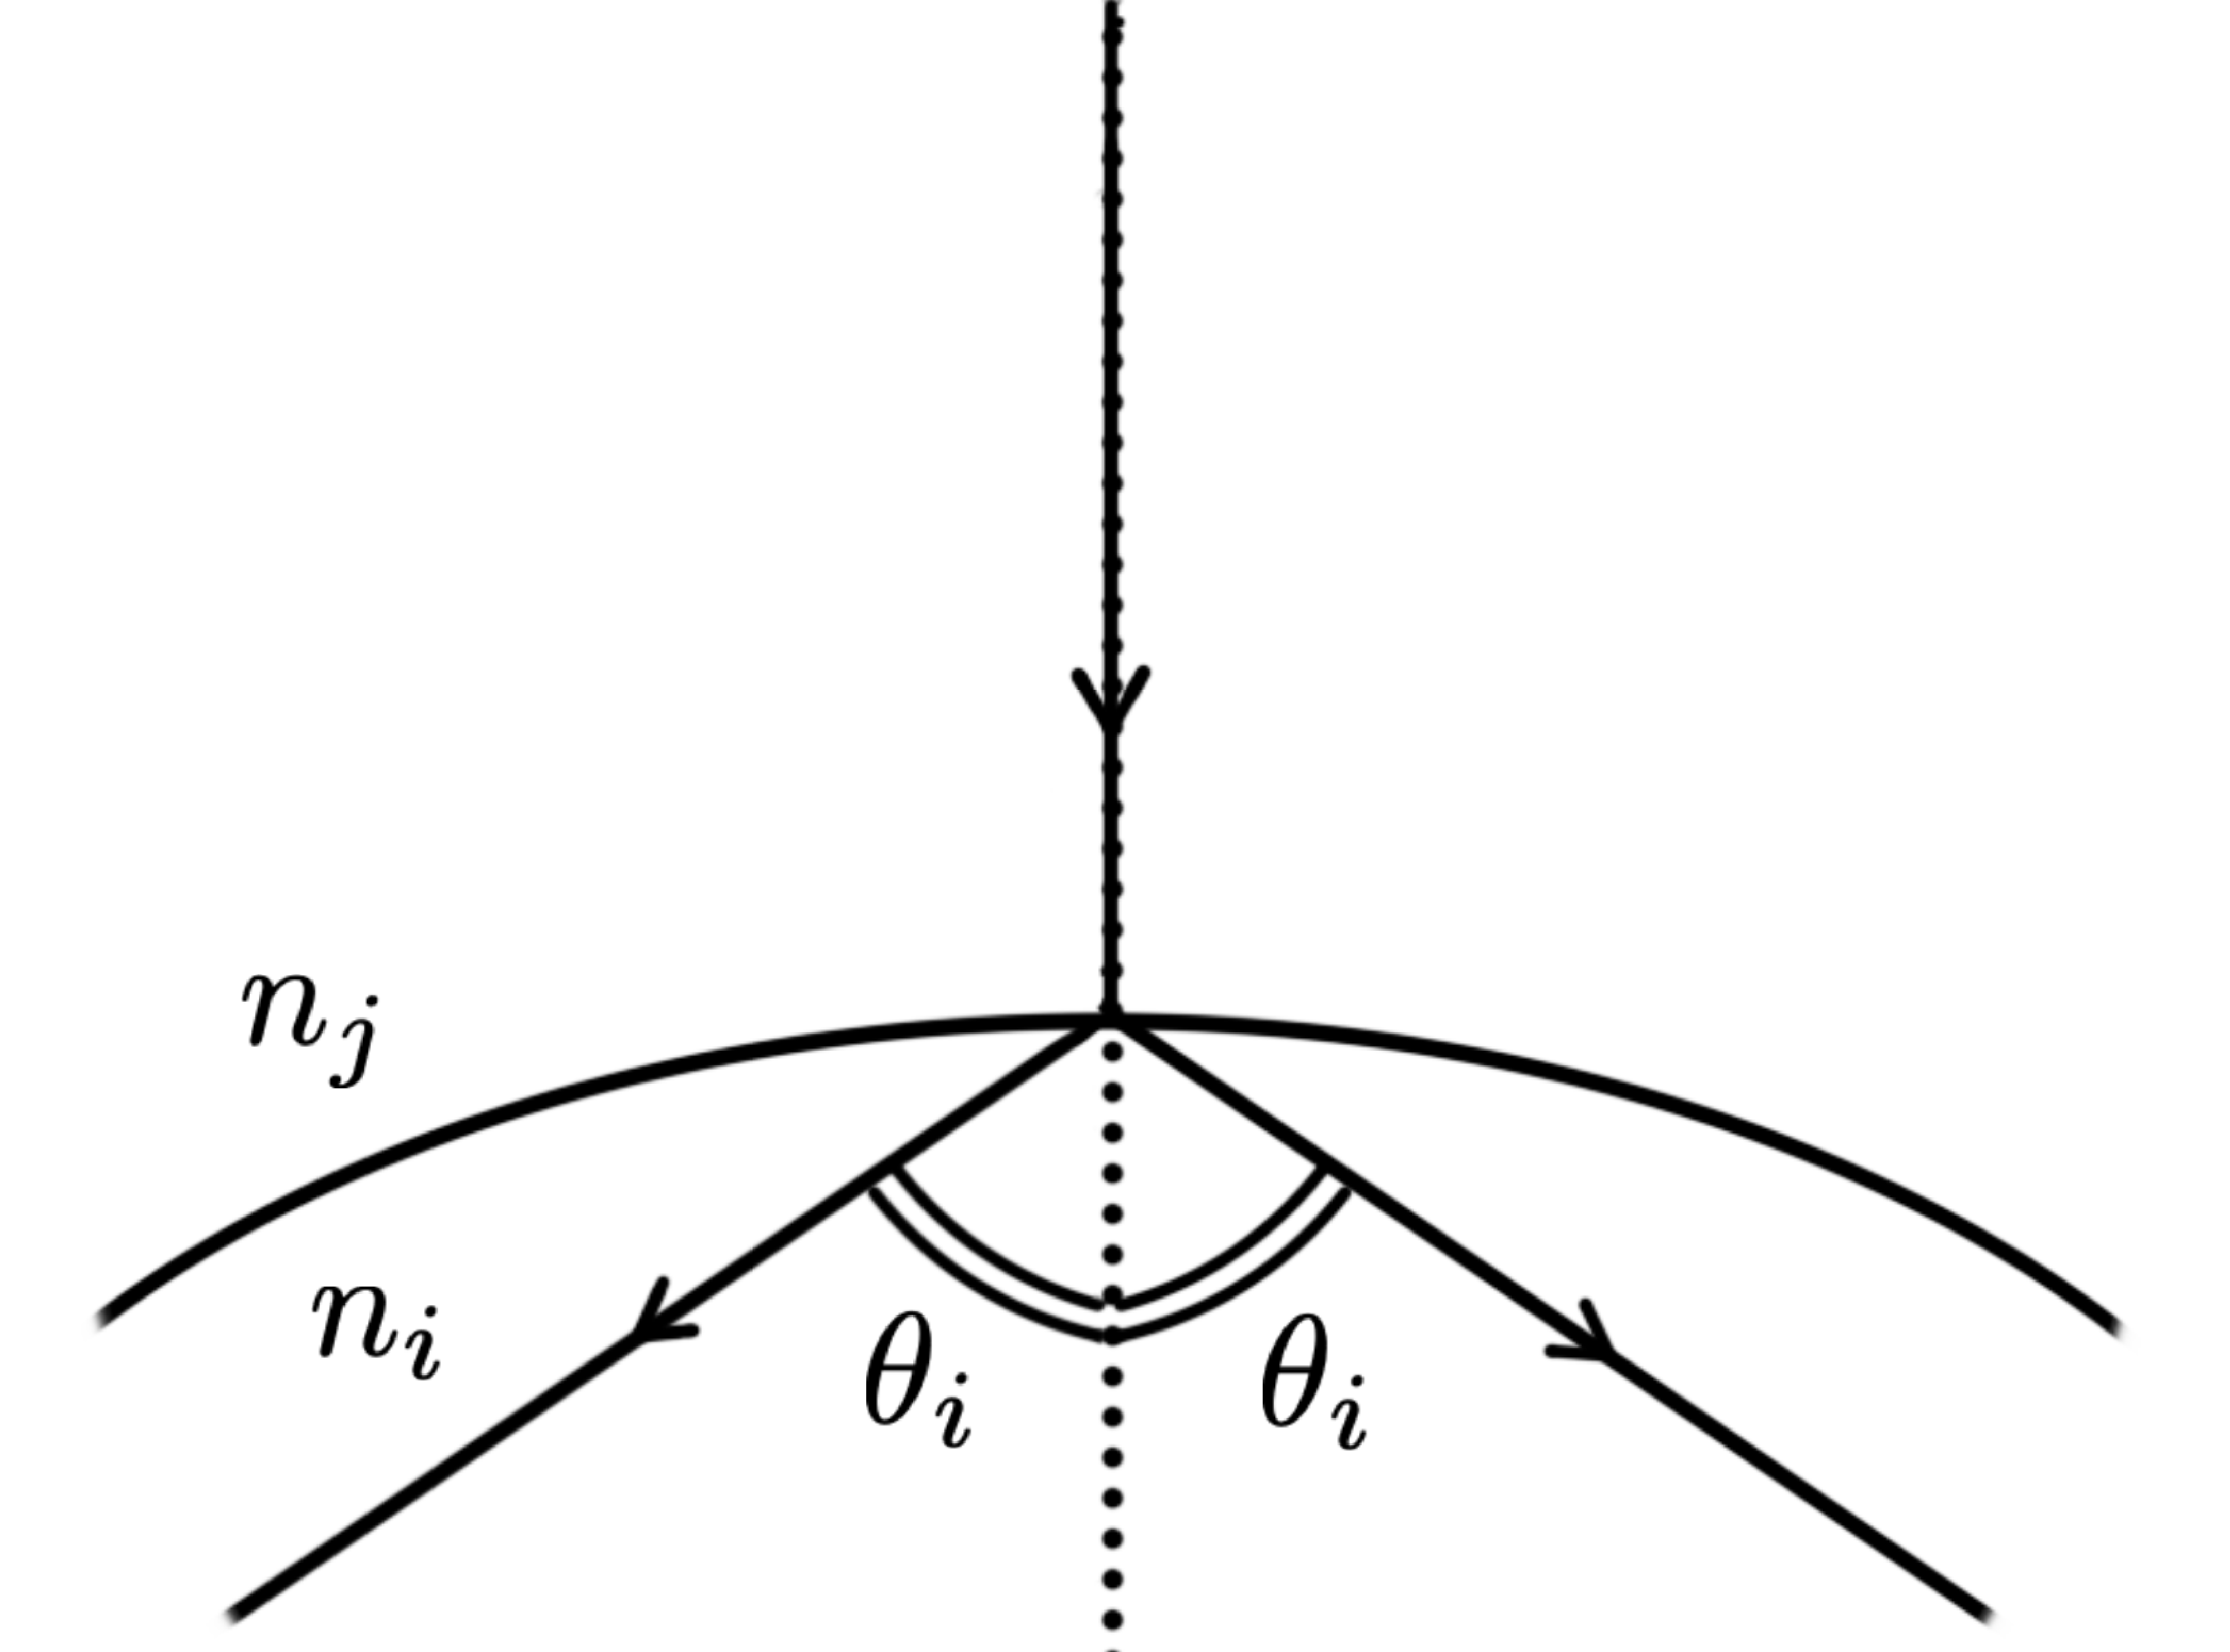
\includegraphics[width=\linewidth]{images/section1/example3.pdf}
    \caption{Иллюстрация к пункту 4.}
    \label{fig:pt8:_example3}
\endminipage\hfill
\end{figure}

Вернемся к рассматриваемой системе в области $\Omega = \Omega_1 \cup \Omega_2$. Определим функцию $\Xi(x, y, v_x, v_y)$ положения и скорости материальной точки (в декартовых координатах) по формуле
\begin{equation*}
\Xi(x, y, v_x, v_y) = \left[
\begin{array}{ll}
    \Lambda(x, y, v_x, v_y) n_1^2, &  \text{ если } (x,y) \in \Omega_1 \\
    \Lambda(x, y, v_x, v_y) n_2^2 + \lambda_1 (n_1^2-n_2^2), & \text{ если } (x,y) \in \Omega_2    .
\end{array}
\right.
\end{equation*}
Здесь величина $\Lambda(x, y, v_x, v_y) =  \dfrac{a^2 v_y^2 + b^2v_x^2 - (x v_y-y v_x)^2}{v_x^2 + v_y^2}$ имеет смысл коэффициента $\alpha$  софокусной квадрики $Q_\alpha$, которая касается прямой, проходящей через точку $(x,y)$ в направлении вектора $(v_x, v_y)$.

Функция $\Xi(x, y, v_x, v_y)$ является первым интегралом рассматриваемой динамической системы в области $\Omega$, см. \cite{vestnikLatest}.

Это утверждение оказывается верным в значительно более общей ситуации.
Пусть внутренность эллипса разбита попарно непересекающимися дугами софокусных квадрик на области $\Omega_1, \ldots, \Omega_k$.  Перенумеруем области так, чтобы общие границы имели только области с соседними номерами. Пусть $\lambda_j$ --- параметр софокусной квадрики, разделяющей $\Omega_j$ и $\Omega_{j+1}$, $j=1, \ldots, k-1$. Два возможных варианта показаны на рис. \ref{fig:pt8:_example4} и \ref{fig:pt8:_example5}. Здесь и далее показатель преломления для области $\Omega_j$ обозначается через $n_j$.
\begin{figure}[!htb]
\minipage{0.45\textwidth}
   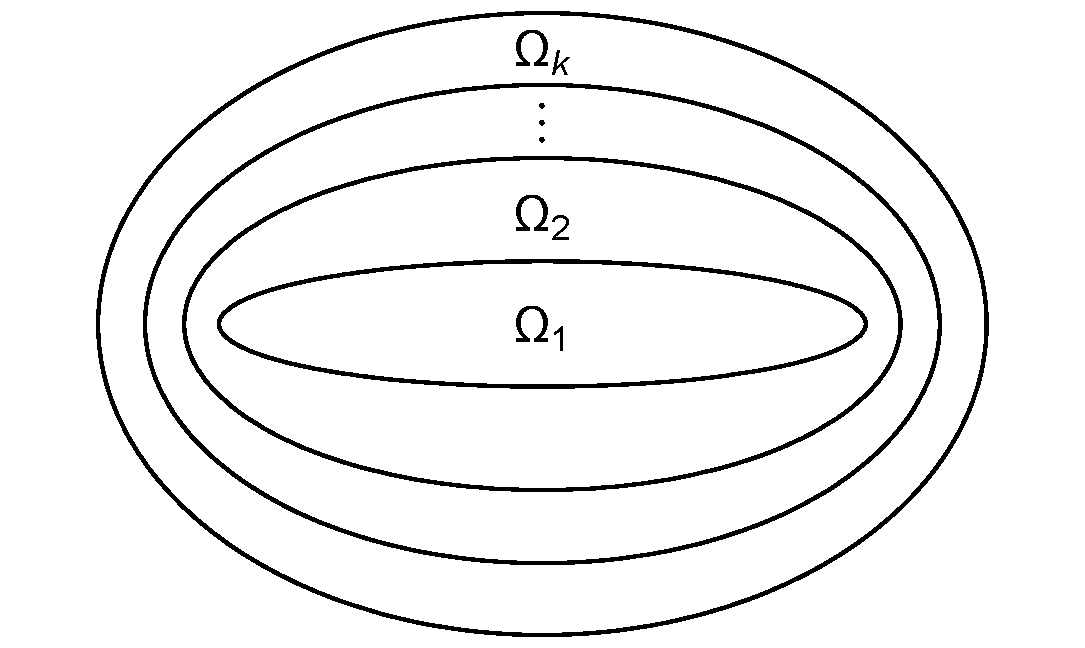
\includegraphics[width=1\textwidth]{images/section1/multiple ellipses.pdf}
    \caption{Взаимное расположение областей $\Omega_1, \ldots, \Omega_k$.}
    \label{fig:pt8:_example4}
\endminipage\hfill
\minipage{0.45\textwidth}
    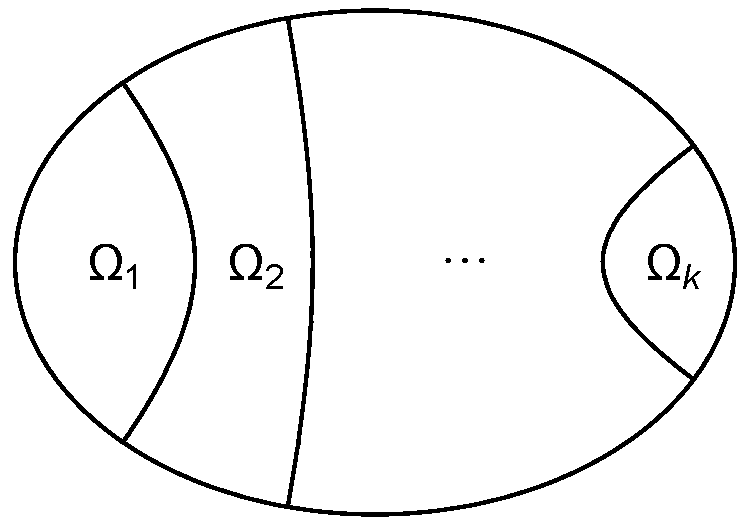
\includegraphics[width=0.9\textwidth]{images/section1/multiple hyperbolas.pdf}   
    \caption{Взаимное расположение областей $\Omega_1, \ldots, \Omega_k$.}
    \label{fig:pt8:_example5}
\endminipage\hfill
\end{figure}


Определим функцию $\Xi(x, y, v_x, v_y)$ по формуле: 
\begin{equation*}
\Xi(x, y, v_x, v_y) = \left[
\begin{array}{ll}
    \Lambda(x, y, v_x, v_y) n_1^2, \qquad  \ \ \qquad   \text{ если } (x,y) \in \Omega_1 
    \\
    \Lambda(x, y, v_x, v_y) n_p^2 + \sum_{j=1}^{p-1} \lambda_j(n_j^2-n_{j+1}^2), \\
     \qquad \qquad \qquad \qquad \qquad \qquad  \text{ если } (x,y) \in \Omega_p \text{ для } 1 < p \leq k. 
\end{array}
\right.
\end{equation*}

\begin{theorem}[\cite{vestnikLatest}]
Функция $\Xi(x, y, v_x, v_y)$ является константой на траекториях бильярда с модифицированным законом  преломления
\end{theorem}

Таким образом, возникает следующая важная естественная задача.

\textbf{Задача А:} описать слоение изоэнергетического многообразия на поверхности уровня первого интеграла $\Xi$ для случаев, показанных на рис. \ref{fig:pt8:_example4} и \ref{fig:pt8:_example5}. 

В работе подробно рассматривается случай двух областей, разделенных одним софокусным эллипсом (см. рис. \ref{fig:pt8:_example4} при $k=2$). Динамика этой системы и перестройки поверхностей постоянного значения интеграла $\Xi$ уже в этом случае очень нетривиальны.
\bigskip

Случаи, когда область $\Omega$ разбивается на подобласти дугами \textit{пересекающихся} софокусных квадрик, оказываются гораздо сложнее. В частности, дополнительный интеграл принимает значения не в $\mathbb{R}$, а в фактор-группе $\mathbb{R}$ по  аддитивной подгруппе, допускающей явное описание.


{\it Случай 1: одна точка пересечения. }

\begin{figure}[!htb]
\centering
     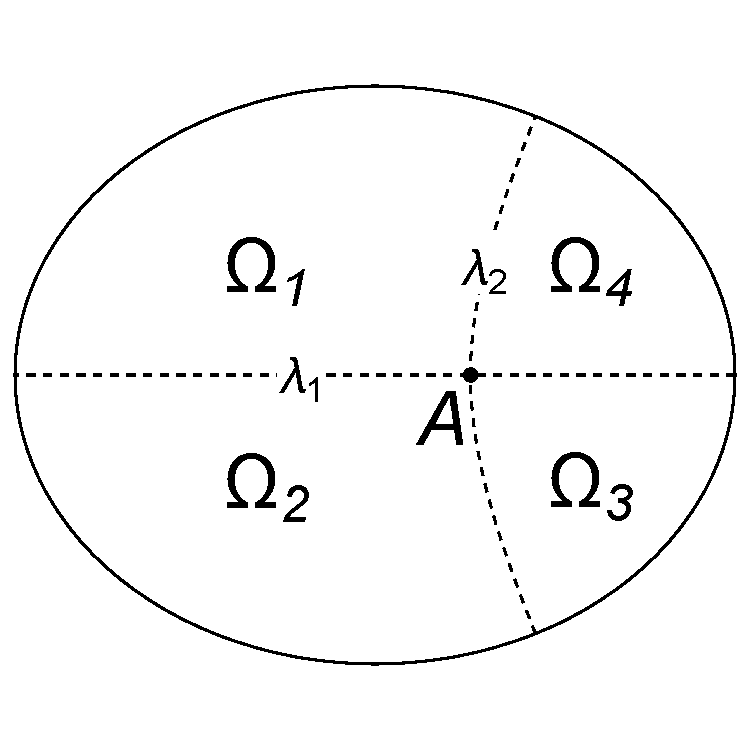
\includegraphics[width=0.35\textwidth]{images/section1/img2.pdf}
\caption{Взаимное расположение областей $\Omega_1,\ldots,\Omega_4$.}
    \label{fig:pt8:_example6}
\end{figure}

Предположим, что внутренность эллипса разделена на области дугами софокусных квадрик таким образом, что имеются всего одна точка их пересечения, которую обозначим $A$.
Занумеруем области против часовой стрелки $\Omega_1, \ \Omega_2, \ \Omega_3, \ \Omega_4$ (см. рис. \ref{fig:pt8:_example6}).
Пусть общая часть границы $\Omega_1 \cup \Omega_4$ и $\Omega_2 \cup \Omega_3$ --- дуга софокусной квадрики с параметром $\lambda_1$, а общая часть границы $\Omega_1 \cup \Omega_2$ и $\Omega_3 \cup \Omega_4$ --- дуга софокусной квадрики с параметром $\lambda_2$ (см. рис. \ref{fig:pt8:_example6}).

Введем коэффициент $\gamma_A$ в точке $A$, имеющий смысл коэффициента ветвления, по формуле $$\gamma_A = \lambda_1(n_1^2 - n_2^2) + \lambda_2(n_2^2-n_3^2) + \lambda_1(n_3^2-n_4^2) + \lambda_2(n_4^2-n_1^2) = (\lambda_1 - \lambda_2) ( n_1^2 - n_2^2 + n_3^2 - n_4^2).$$

Определим вспомогательную функцию $\widetilde{\Xi}(x, y, v_x, v_y)$ 

\begin{equation*}
\widetilde{\Xi}(x, y, v_x, v_y) = \left[
\begin{array}{ll}
    \Lambda(x, y, v_x, v_y) n_1^2, \qquad  \  \ \qquad   \text{ если } (x,y) \in \Omega_1 
    \\
    \Lambda(x, y, v_x, v_y) n_p^2 + \sum_{j=1}^{p-1} \lambda_j(n_j^2-n_{j+1}^2), \\
     \qquad \qquad \qquad \qquad \qquad \qquad  \text{ если } (x,y) \in \Omega_p \text{ для } 1 < p \leq 4. 
\end{array}
\right.
\end{equation*}
Неформально говоря, она почти подходит на роль дополнительного интеграла, но имеет разрыв на дуге, разделяющей области $\Omega_1$ и $\Omega_4$. Можно проверить, что на любой бильярдной траектории, пересекающей эту дугу, функция $\widetilde{\Xi}$ испытывает один и тот же скачок, равный  $\pm \gamma_A$. 
Поэтому мы определим \textit{первый интеграл $\Xi(x, y, v_x, v_y)$ со значениями в $S^1= \mathbb{R}/\gamma_A \mathbb{Z}$ }по формуле $$\Xi(x, y, v_x, v_y) = \widetilde{\Xi}(x, y, v_x, v_y) \mod \gamma_A.$$
Эта величина на траекториях бильярда сохраняется.
\bigskip

Если границы раздела областей пересекаются по двум и более точкам, то имеет место общая закономерность: 
\medskip

{\it 
\noindent Для каждой точки пересечения $A_i, i=1,\ldots,m$, определен коэффициент $\gamma_{A_i}$. Дополнительный интеграл \  $\Xi(x, y, v_x, v_y)$ принимает значения в $\mathbb{R}/(\gamma_{A_1} \mathbb{Z}+ \ldots + \gamma_{A_m} \mathbb{Z})$. Если $\gamma_{A_i}$ соизмеримы, т. е. всевозможные дроби $\dfrac{\gamma_{A_i}}{\gamma_{A_j}}$ --- рациональные числа (или бесконечность), то $\mathbb{R}/(\gamma_{A_1} \mathbb{Z}+ \ldots + \gamma_{A_m} \mathbb{Z}) = S^1$. Если же среди $\gamma_{A_i}$ есть пара с иррациональным отношением $\dfrac{\gamma_{A_i}}{\gamma_{A_j}}$, то подгруппа $\gamma_{A_1} \mathbb{Z}+ \ldots + \gamma_{A_m} \mathbb{Z}$ всюду плотна в $\mathbb{R}$. В этом случае дополнительный интеграл $\Xi(x, y, v_x, v_y)$ корректно определен, но использовать его для топологического анализа структуры траекторий представляется весьма затруднительным.}

\bigskip
{\it Случай 2: две точки пересечения.}
\begin{figure}[!htb]
\centering
   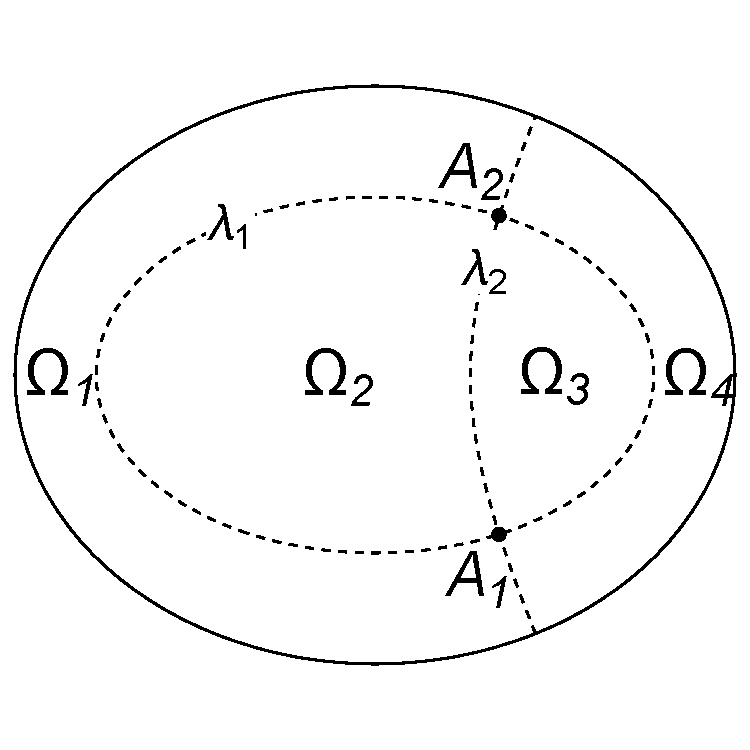
\includegraphics[width=0.35\textwidth]{images/section1/img3.pdf}   
    \caption{Взаимное расположение областей $\Omega_1, \ldots, \Omega_4$.}
    \label{fig:pt8:_example7}
\end{figure}
Рассмотрим области, изображенные на рис. \ref{fig:pt8:_example7}. 
Легко вычислить коэффициенты $\gamma_{A_1}$ и $\gamma_{A_2}$ в точках $A_1, A_2$ (т.е. скачки дополнительного интеграла при обходе против часовой стрелки вокруг соответствующей точки):
$$\gamma_{A_1} = \lambda_2(n_1^2 - n_4^2) + \lambda_1(n_4^2-n_3^2) + \lambda_2(n_3^2-n_2^2) + \lambda_1(n_2^2-n_4^2), $$
% = (\lambda_2 - \lambda_1) ( n_1^2 - n_2^2 + n_3^2 - n_4^2),$$
$$\gamma_{A_2} = \lambda_1(n_1^2 - n_2^2) + \lambda_2(n_2^2-n_3^2) + \lambda_1(n_3^2-n_4^2) + \lambda_2(n_4^2-n_1^2). $$
% = (\lambda_1 - \lambda_2) ( n_1^2 - n_2^2 + n_3^2 - n_4^2).$$
Как видно, в этом случае $$\gamma_{A_1} = -\gamma_{A_2}.$$
Поэтому дополнительный интеграл $\Xi(x, y, v_x, v_y)$, сохраняющийся на траекториях бильярда, может быть задан по модулю $\gamma_{A_1}$ формулой $\Xi = \widetilde{\Xi} \mod \gamma_{A_1}$, где 
\begin{equation*}
\widetilde{\Xi}(x, y, v_x, v_y) = \left[
\begin{array}{ll}
    \Lambda(x, y, v_x, v_y) n_1^2,  \qquad \ \  \qquad  \text{ если } (x,y) \in \Omega_1 
    \\
    \Lambda(x, y, v_x, v_y) n_p^2 + 
    \sum_{j=1}^{p-1} \lambda_j(n_j^2-n_{j+1}^2), \\
     \qquad \qquad  \qquad \qquad  \qquad \qquad \text{ если } (x,y) \in \Omega_p \text{ для } 1 < p \leq 4. 
\end{array}
\right.
\end{equation*}
 \medskip
{\it Случай 3: две точки пересечения.}
Рассмотрим области, изображенные на рис. \ref{fig:pt8:_example8}. 
\begin{figure}[!htb]
\centering
   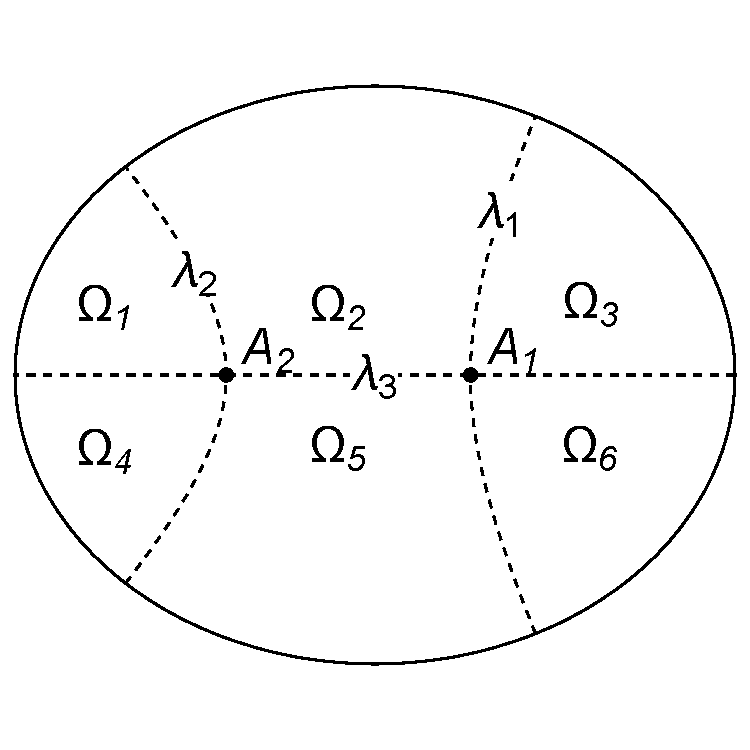
\includegraphics[width=0.35\textwidth]{images/section1/img4.pdf}   
    \caption{Взаимное расположение областей $\Omega_1, \ldots, \Omega_6$.}
    \label{fig:pt8:_example8}
\end{figure}


Легко видеть, что коэффициенты $\gamma_{A_1}, \gamma_{A_2}$ в точках $A_1$, $A_2$, соответственно, задаются формулами:
$$\gamma_{A_1} = (\lambda_3 - \lambda_1)(n_2^2 - n_5^2 + n_6^2 - n_3^2),$$
$$\gamma_{A_2} = (\lambda_3 - \lambda_2)(n_1^2 - n_4^2 + n_5^2 - n_2^2).$$

В зависимости от значений параметров отношение $\dfrac{\gamma_{A_1}}{\gamma_{A_2}}$ может быть как рациональным, так и иррациональным.

Роль коэффициента $\gamma_A$ проявляется в следующей задаче, которую мы решим в рамках настоящей статьи.

\textbf{Задача Б.} Рассмотрим в качестве бильярдной области $\Omega$  <<прямоугольник>>, образованный дугами концентрических окружностей $BC$, $AD$ и отрезками вертикально проведенного диаметра $AB$ и $CD$. (см. рис. \ref{fig:pt8:_example9}).
Область $\Omega$ разбивается на две части дугой  $EF$ концентрической окружности  и отрезком $FG$ горизонтально проведенного диаметра. Нумерация областей показана на рис. \ref{fig:pt8:_example9}.

Требуется описать как изоэнергетическое многообразие расслаивается на поверхности уровня первого интеграла $\Xi$.


\begin{figure}[!htb]
\centering
   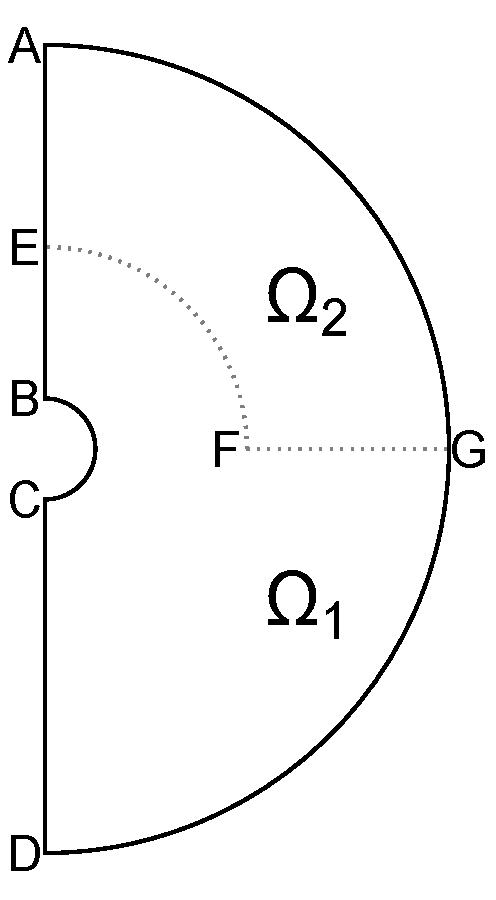
\includegraphics[width=0.25\textwidth]{images/section1/imgB.pdf}   
    \caption{Взаимное расположение областей $\Omega_1, \Omega_2$.}
    \label{fig:pt8:_example9}
\end{figure}

Перечислим основные результаты настоящей работы.
Для задачи А полностью описаны поверхности уровня регулярных значений интеграла $\Xi$ (теорема \ref{st:pt9:n1_n2_surfaces}).
В разделе \ref{s2.1.2}  описаны поверхности уровня для всех нерегулярных значений интеграла $\Xi$, а также все перестройки поверхностей уровня интеграла при проходе через сингулярные значения. 
Для задачи Б  показано, что многозначный интеграл $\Xi$ в действительности принимает лишь конечное число значений, в теоремах \ref{th:pt10:th1} и \ref{th:pt10:th2} и подразделе \ref{s3.8} полностью описаны поверхности уровня регулярных значений интеграла $\Xi$.
Описанию особых слоев и перестроек посвящен подраздел \ref{s3.10}.
\bigskip

